% Using Epistemic Observability in Agentic Systems for Combating Hallucinations
% PACMI '26 workshop talk: 12 minutes + 3 minutes questions
% Build: make            (slides)
%        make notes      (slides with speaker notes on the right)
%
% Figures are read from ../../papers/pacmi26/figures so the slides cannot
% drift from the paper: regenerate there, rebuild here.

\documentclass[aspectratio=169,10pt]{beamer}

\usetheme{metropolis}
\metroset{progressbar=none, numbering=fraction, block=fill}
\setbeamertemplate{navigation symbols}{}
\setbeamertemplate{frame footer}{PACMI '26 \quad Mason \& Anand}
\setbeamerfont{frame footer}{size=\tiny}

\usepackage{graphicx}
\graphicspath{{../../papers/pacmi26/figures/}}
\usepackage{booktabs}
\usepackage{amsmath,amssymb}
\usepackage{tikz}
\usetikzlibrary{arrows.meta,positioning,calc}
\usepackage{xcolor}
\usepackage{qrcode}
\usepackage{pgfpages}
\ifdefined\shownotes
  \setbeameroption{show notes on second screen=right}
\fi

% Palette shared with the paper: entropy white (confident) -> deep red (uncertain)
\definecolor{ent0bg}{rgb}{1,1,1}
\definecolor{ent0fg}{rgb}{0,0,0}
\definecolor{ent1bg}{rgb}{0.97,0.97,0.97}
\definecolor{ent1fg}{rgb}{0,0,0}
\definecolor{ent2bg}{rgb}{0.85,0.85,0.85}
\definecolor{ent2fg}{rgb}{0,0,0}
\definecolor{ent3bg}{rgb}{1,0.78,0.78}
\definecolor{ent3fg}{rgb}{0,0,0}
\definecolor{ent4bg}{rgb}{1,0.47,0.47}
\definecolor{ent4fg}{rgb}{1,1,1}
\definecolor{ent5bg}{rgb}{0.86,0.19,0.19}
\definecolor{ent5fg}{rgb}{1,1,1}
\definecolor{ent6bg}{rgb}{0.62,0,0}
\definecolor{ent6fg}{rgb}{1,1,1}
\newcommand{\etok}[2]{\colorbox{ent#1bg}{\strut\textcolor{ent#1fg}{\texttt{#2}}}\hspace{-0.5pt}}

% IBM colorblind-safe pair used in the paper figures
\definecolor{knowable}{HTML}{FE6100}
\definecolor{unknowable}{HTML}{785EF0}
\definecolor{tensorblue}{HTML}{648FFF}
\definecolor{textpink}{HTML}{DC267F}

\newcommand{\pp}[1]{\textbf{#1\,pp}}

\title{Using Epistemic Observability in Agentic Systems\\for Combating Hallucinations}
\author{Tony Mason\inst{1} \and Vaastav Anand\inst{2}}
\institute{\inst{1}The University of British Columbia \qquad \inst{2}Max Planck Institute for Software Systems}
\date{PACMI '26 \quad Prague}

\begin{document}

\maketitle
\note{0:00. One sentence: this talk is about what a system can learn about a
language model's output if the model exposes more than text, and what that is
worth per unit of verification budget.}

%------------------------------------------------------------------------------
\begin{frame}{Which ten percent do you check?}
  \begin{itemize}
    \item Some fraction of every model's output is fabricated: fluent, confident, wrong.
      Fabrication is provably inevitable for LLMs over computable functions
      (Xu et al.\ 2024). It is the expected behaviour of coherence optimisation,
      not a malfunction.
    \item Verification is not free. A citation lookup costs latency. A judge model
      costs compute. A human costs both, and costs the automation.
    \item So every deployment already allocates a budget: how much to verify, in
      what order, using what signal to choose.
  \end{itemize}
  \vspace{0.5em}
  \begin{block}{The systems question}
    If the model exposed more than its text, what would that buy per unit of
    verification budget?
  \end{block}
  \note{1:00. Land the framing: this is a budget-allocation problem, and the
  paper is a cost surface, not a detector. Do not say "hallucination" without
  "fabrication" beside it; the word choice is deliberate.}
\end{frame}

%------------------------------------------------------------------------------
\begin{frame}{The observability gap}
  \begin{columns}[T]
    \begin{column}{0.52\textwidth}
      \centering
      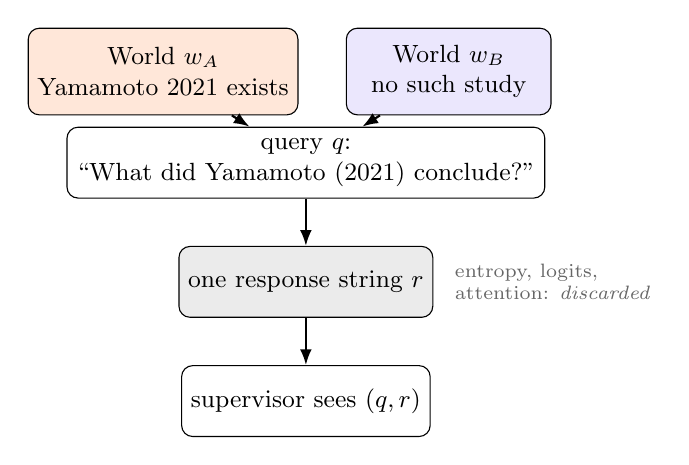
\begin{tikzpicture}[
          world/.style={draw, rounded corners, minimum width=2.6cm, minimum height=1.1cm, align=center, font=\small},
          box/.style={draw, rounded corners, minimum width=2.6cm, minimum height=0.9cm, align=center, font=\small},
          arr/.style={-{Latex[length=2mm]}, thick}]
        \node[world, fill=knowable!15] (wa) {World $w_A$\\Yamamoto 2021 exists};
        \node[world, fill=unknowable!15, right=0.6cm of wa] (wb) {World $w_B$\\no such study};
        \node[box, below=0.7cm of $(wa)!0.5!(wb)$] (q) {query $q$:\\``What did Yamamoto (2021) conclude?''};
        \node[box, fill=black!8, below=0.6cm of q] (r) {one response string $r$};
        \node[box, below=0.6cm of r] (s) {supervisor sees $(q, r)$};
        \draw[arr] (wa) -- (q);
        \draw[arr] (wb) -- (q);
        \draw[arr] (q) -- (r);
        \draw[arr] (r) -- (s);
        \node[font=\scriptsize, text=black!60, align=left, right=0.15cm of r] {entropy, logits,\\attention: \emph{discarded}};
      \end{tikzpicture}
    \end{column}
    \begin{column}{0.46\textwidth}
      \small
      \begin{itemize}
        \item Honesty asks for an answer in $w_A$ and an abstention in $w_B$.
          The supervisor receives the same string in both.
        \item Under bounded supervision, grounded and fabricated states can be
          observationally equivalent through text, whatever the scale or
          training (Mason \& Anand, arXiv 2026).
        \item The signals that could tell them apart were computed during
          generation and discarded at the interface. The supervisor pays to
          reconstruct them.
      \end{itemize}
    \end{column}
  \end{columns}
  \note{2:30. This is the claim the whole talk rests on, so say it as a claim
  about the observer, not about the model: from text alone, a bounded observer
  cannot verify. The formal version is in the arXiv paper; here it is the
  motivation for the interface. Do not overstate it as "honesty is impossible".}
\end{frame}

%------------------------------------------------------------------------------
\begin{frame}{The cheapest fix: ask the model}
  \begin{columns}[T]
    \begin{column}{0.58\textwidth}
      
\includegraphics[width=\textwidth]{exp27_confidence_distributions.pdf}
    \end{column}
    \begin{column}{0.42\textwidth}
      \small
      ``How confident are you?'', asked after generation. Four
      instruction-tuned families, 200 queries each.
      \begin{itemize}
        \item Mean self-report \textcolor{knowable}{\textbf{0.98}} knowable,
          \textcolor{unknowable}{\textbf{0.73}} unknowable.
        \item 43\% of unknowable queries: a literal ``100''.
        \item The ordering exists (AUC 0.66--0.92) but the scale is compressed
          into its top end. A threshold that admits the correct answers admits
          the fabrications too.
      \end{itemize}
      \vspace{0.2em}
      Self-report is \emph{testimony}: produced by the objective that produced
      the answer.
  \end{column}
  \end{columns}
  \note{4:00. Point at Llama and Mistral: almost every response, knowable or
  not, sits at 1.0. The CDF was Vaastav's change and it reads better than the
  histogram did: the separation is visible in OLMo and Qwen, and it is still
  useless as a threshold. Numbers are from the corrected parse (Chris Brew's
  fix); the old inversion claim is retracted and must not be said.}
\end{frame}

%------------------------------------------------------------------------------
\begin{frame}{Testimony and telemetry}
  \begin{columns}[T]
    \begin{column}{0.46\textwidth}
      \textbf{Testimony}: the generated text. Optimised to satisfy the prompt,
      so it can mislead by construction.

      \vspace{0.5em}
      \textbf{Telemetry}: byproducts of inference the model does not choose to
      emit: per-token entropy, log-probabilities, attention statistics. Under
      current training, changing them means changing the computation.

      \vspace{0.5em}
      \textbf{Epistemic observability}: export the telemetry with the text so
      a downstream system can estimate fabrication risk. Not interpretability
      (why), not explainability (post-hoc rationale).
    \end{column}
    \begin{column}{0.54\textwidth}
      \footnotesize
      \begin{tabular}{@{}lll@{}}
        \toprule
        Tier & Exposes & Cost \\
        \midrule
        0 Output & text only (today's APIs) & external checks \\
        1 Confidence & logprobs, entropy & negligible \\
        2 Representation & hidden states, probes & moderate \\
        3 Mechanistic & circuits, information flow & high \\
        \bottomrule
      \end{tabular}
      \vspace{0.3em}

      \small A brainstorming tool needs Tier~0. Medical decision support may
      justify Tier~2 or~3. The hierarchy says what each level of investment buys.
    \end{column}
  \end{columns}
  \note{5:30. Two words to make stick: testimony and telemetry. The tier table
  is the paper's organising contribution; the rest of the talk lives at Tier~1
  with one cheap Tier~2 signal that the evaluation does not use.}
\end{frame}

%------------------------------------------------------------------------------
\begin{frame}{A minimal tensor interface}
  \small
  \textbf{What shape is wombat scat?} \hfill entropy: \etok{0}{\ low\ }\etok{1}{\ \ }\etok{2}{\ \ }\etok{3}{\ mid\ }\etok{4}{\ \ }\etok{5}{\ \ }\etok{6}{\ high\ }

  \vspace{0.4em}
  \noindent\etok{0}{W}\etok{1}{ombat}\etok{0}{ sc}\etok{0}{at}\etok{2}{ is}\etok{2}{ typically}\etok{4}{ cylindrical}\etok{3}{ or}\etok{5}{ sausage}\etok{0}{-shaped}\etok{1}{.}\etok{2}{ This}\etok{3}{ form}\etok{1}{ helps}\etok{2}{ the}\etok{2}{ sc}\etok{0}{at}\etok{3}{ to}\etok{1}{ be}\etok{2}{ easily}\etok{5}{ transported}\etok{4}{ by}\etok{2}{ wind}\etok{3}{ or}\etok{6}{ through}\etok{2}{ the}\etok{6}{ soil}\etok{3}{,}\etok{4}{ aiding}\etok{0}{ in}\etok{3}{ dispers}\etok{0}{al}\etok{2}{ and}\etok{5}{ preventing}\etok{5}{ it}\etok{0}{ from}\etok{4}{ being}\etok{6}{ easily}\etok{6}{ eaten}\etok{0}{ by}\etok{1}{ predators}\etok{2}{.}

  \vspace{0.1em}
  \textit{Wombat scat is cube-shaped. The answer is a fabrication, and the model was uncertain exactly where it was inventing.}

  \vspace{0.3em}
  \begin{columns}[T]
    \begin{column}{0.48\textwidth}
      \textbf{Returns}: text, per-token entropy trace, attention summary.\\
      No architectural change: the logits already exist.\\
      Overhead 2--7\% latency over generation.
    \end{column}
    \begin{column}{0.48\textwidth}
      \textbf{Is not}: a lie detector. Low entropy does not mean true.
      Entropy conflates epistemic uncertainty with aleatoric spread.\\
      It \emph{ranks} outputs for verification. It does not classify them.
    \end{column}
  \end{columns}
  \note{7:00. Read the trace aloud: confident on "Wombat scat is", uncertain
  on "cylindrical", "sausage", "through the soil", "easily eaten". The
  evaluation uses entropy alone; make no claim about what attention adds.}
\end{frame}

%------------------------------------------------------------------------------
\begin{frame}{Evaluation: return on verification investment}
  \begin{columns}[T]
    \begin{column}{0.5\textwidth}
      \textbf{Queries}: 100 knowable, 100 unknowable (nonexistent people,
      fictional syndromes, future events, fake citations). Labels by construction.

      \vspace{0.4em}
      \textbf{Models}: OLMo-3 7B, Llama-3.1 8B, Qwen3 4B, Mistral 7B, all
      instruction-tuned. 800 responses.

      \vspace{0.4em}
      \textbf{Budgets}: the judge may verify 10\%, 20\%, or 30\% of outputs.
      Confirmed fabrications become abstentions.
    \end{column}
    \begin{column}{0.5\textwidth}
      \textbf{Four judges}
      \begin{enumerate}
        \item No judge: raw output.
        \item \textcolor{textpink}{Text-guided}: rank by response word count.
        \item \textcolor{tensorblue}{Tensor-guided}: rank by mean entropy.
        \item Composed: tensor ranking, plus an \emph{oracle} for citation-like queries.
      \end{enumerate}
      \vspace{0.4em}
      \small
      Verification is simulated (1{,}000 seeded trials): a selected fabrication is
      caught with $p=0.938$, a selected error corrected with $p=0.95$. The 0.938
      is evaluator agreement with a blinded 80-item author review, used as a
      parameter, not a measured catch rate.
    \end{column}
  \end{columns}
  \note{8:00. Say the simulation parameters out loud before anyone asks. The
  length baseline is the strongest text-channel signal we found, which is why
  it is the comparison and not a straw man.}
\end{frame}

%------------------------------------------------------------------------------
\begin{frame}{Tensor-guided verification wins at every budget}
  \begin{columns}[T]
    \begin{column}{0.54\textwidth}
      
\includegraphics[width=\textwidth]{exp27_aggregate_budget_curve.pdf}
      \footnotesize
      Per family at 10\%, over no judge: OLMo 69.5\,$\to$\,75.1, Llama
      82.5\,$\to$\,88.1, Qwen 87.0\,$\to$\,91.7, Mistral 64.0\,$\to$\,72.0.
    \end{column}
    \begin{column}{0.46\textwidth}
      \small
      800 responses pooled under one budget: \pp{+3.3}, \pp{+4.6}, \pp{+3.3}
      over the length judge at 10/20/30\%.

      \vspace{0.4em}
      \textbf{What we do not claim.}
      \begin{itemize}
        \item That entropy is the better \emph{detector}. Length ranks at AUC
          0.85--0.97 and beats entropy on two of four families.
        \item The gain comes from \emph{which items} each signal selects.
          Mistral at 30\%: length wins by 2.2\,pp.
        \item The composed judge reads the ground-truth label for citation
          queries: the headroom a perfect lookup would buy, not a result.
      \end{itemize}
    \end{column}
  \end{columns}
  \note{9:30. Give the caveats the same time as the headline. A reviewer who
  hears "entropy beats length" will check and find otherwise. The honest
  version is: two signals, different items, and one of them the model can be
  trained to move without touching the computation. That is the next slide.}
\end{frame}

%------------------------------------------------------------------------------
\begin{frame}{Why prefer telemetry when a text signal is this good?}
  \begin{columns}[T]
    \begin{column}{0.5\textwidth}
      \textbf{Coupling.} Length and hedging are surface regularities; training
      can move them without touching the computation beneath. The entropy
      trace moves only if the computation does. It is not \emph{separately}
      controllable from the thing being monitored.

      \vspace{0.4em}
      \small
      Holds under current pipelines. A monitor inside the training objective
      is a different regime; we claim nothing about it. Exporting the telemetry
      at least makes that manipulation auditable.
    \end{column}
    \begin{column}{0.5\textwidth}
      \textbf{Does post-training erase it?} Four public OLMo-3 checkpoints:
      base, SFT, DPO, RLVR.
      \begin{itemize}
        \item Knowable-query entropy: 1.18\,$\to$\,0.18 nats.
        \item Surviving fabrications: 1.49\,$\to$\,0.98, holding through RLVR.
        \item Separation \emph{widens}: AUC 0.67\,$\to$\,1.00 on 48 probes;
          0.63\,$\to$\,0.81--0.87 with the true-but-implausible category counted.
        \item Refusals on fabrication prompts: 0\%\,$\to$\,56\%.
      \end{itemize}
      \small The widening is robust. The perfect ceiling is not.
    \end{column}
  \end{columns}
  \note{10:45. The wombat in the trace slide belongs to the excluded category,
  so say the 0.81--0.87 figure, not just the 1.00. Post-training makes the
  testimony better and leaves the telemetry usable; that is the finding.}
\end{frame}

%------------------------------------------------------------------------------
\begin{frame}{In a runtime: observe, then decide}
  \begin{columns}[T]
    \begin{column}{0.48\textwidth}
      The interface exposes \emph{evidence}. A deployment policy chooses the
      \emph{action}. Keeping those separate is the design.

      \vspace{0.4em}
      \textbf{Action ladder}, increasing cost:
      abstain or flag \,$\to$\, regenerate \,$\to$\, tool verification \,$\to$\,
      escalate to a higher tier \,$\to$\, human review.
    \end{column}
    \begin{column}{0.52\textwidth}
      \textbf{Three integration points}
      \begin{itemize}
        \item \textbf{Serving layer}: telemetry exported with the text, amount set
          by the tier.
        \item \textbf{Composition boundary}: where the runtime intercepts tool and
          sub-agent calls, telemetry gates propagation. An unverified fabrication in
          step 3 of an agent is input to step 4.
        \item \textbf{Policy layer}: a budget allocator maps telemetry to actions
          from deployment-specific costs.
      \end{itemize}
    \end{column}
  \end{columns}
  \note{11:30. This is the PACMI audience's slide: the evaluation is
  single-step, and the multi-step case is where the gating matters and where
  we have not yet measured.}
\end{frame}

%------------------------------------------------------------------------------
\begin{frame}{What this is, and the ask}
  \begin{columns}[T]
    \begin{column}{0.5\textwidth}
      \textbf{Not claimed}
      \begin{itemize}
        \item Unfakeable under adversarial training.
        \item That tensor signals survive composition in recursive pipelines.
        \item Optimality. We show existence.
        \item Closed-weight models: five further API endpoints (4B--235B,
          top-5 logprobs only) give AUC 0.65--0.88, but providers that export
          no logprobs remain untested.
      \end{itemize}
    \end{column}
    \begin{column}{0.5\textwidth}
      \textbf{Signal access is a provider choice, and it is eroding.}
      Log-probabilities were on early completion endpoints and are absent from
      the newest reasoning models, the systems whose output is hardest to verify.

      \vspace{0.4em}
      When only the provider can see the telemetry, only the provider can
      verify. Everyone downstream pays to reconstruct it.

      \vspace{0.4em}
      \begin{block}{The ask}
        Export the telemetry. It already exists; the interface is the only
        thing discarding it.
      \end{block}
    \end{column}
  \end{columns}
  \note{12:00. End on the ask. If short on time, drop the runtime slide, not
  this one.}
\end{frame}

%------------------------------------------------------------------------------
\begin{frame}{Summary}
  \begin{columns}[T]
    \begin{column}{0.66\textwidth}
      \begin{enumerate}
        \item From text alone, a bounded observer cannot verify. Self-report is
          testimony and reads ``100'' either way.
        \item Epistemic observability: export the telemetry inference already
          produces, in tiers priced by what they cost.
        \item A Tier-1 entropy trace, 2--7\% overhead, buys \pp{+3.3} to \pp{+4.6}
          end-to-end accuracy over the best text signal at every budget, across four
          families, and survives post-training.
      \end{enumerate}
      \vspace{0.5em}
      \small
      Artifact: \url{https://github.com/fsgeek/pacmi26-observability}\\
      DOI 10.5281/zenodo.22162419 (v1.0.7) \quad
      Theory: arXiv, Mason \& Anand 2026
    \end{column}
    \begin{column}{0.3\textwidth}
      \centering
      \qrcode[height=2.6cm]{https://doi.org/10.5281/zenodo.22162419}\\
      \scriptsize artifact
    \end{column}
  \end{columns}
\end{frame}

%==============================================================================
\appendix
\begin{frame}{Backup: the claim, precisely}
  \footnotesize
  \textbf{Bounded supervisor.} Observes $Obs(q,r,w) = (q, r, \mathit{verify}(r,w))$
  when the verification cost is within budget $B$, and $(q, r, \emptyset)$ otherwise.

  \vspace{0.4em}
  \textbf{Hallucination regime.} There is a plausible fabrication $r_{fab}$ and
  worlds $w_A$ (answerable), $w_B$ (not) with verification cost above $B$ in both,
  so $Obs(q, r_{fab}, w_A) = Obs(q, r_{fab}, w_B)$.

  \vspace{0.4em}
  \textbf{Verification impossibility.} Under that regime no bounded supervisor
  observing only text can return a verdict that is correct in both worlds; and
  no learning algorithm driven by that supervisor's reward can be guaranteed to
  converge to a policy that answers in $w_A$ and abstains in $w_B$.

  \vspace{0.4em}
  \textbf{Stacking judges} that consume only the previous judge's output cannot
  add information (observation monotonicity). Triage that re-inspects the
  original artifact, or any interface that exports state between layers, leaves
  the text-only class.

  \vspace{0.4em}
  Mechanised in Lean; TLA+ models of both the text-only regime and the tensor
  interface, model-checked with TLC. In the tensor model \emph{Verifiability}
  still fails at the plausible-lie case, where fluent fabrication and honest
  refusal are both low-entropy and coherent. That residue is the formal
  counterpart of AUC 0.87 rather than 1.0.
\end{frame}

\begin{frame}{Backup: per-family and API results}
  \small
  \begin{columns}[T]
    \begin{column}{0.5\textwidth}
      \textbf{Local, per family, own budget}\\
      Tensor over no judge at 10\%: OLMo 69.5\,$\to$\,75.1, Llama
      82.5\,$\to$\,88.1, Qwen 87.0\,$\to$\,91.7, Mistral 64.0\,$\to$\,72.0.\\
      Tensor over length, averaged: +2.6 / +3.9 / +2.6\,pp at 10/20/30\%.\\
      Mistral at 30\%: length wins by 2.2\,pp.

      \vspace{0.4em}
      \textbf{Detector AUC, knowable vs.\ unknowable}\\
      Entropy 0.87--0.92 per family.\\
      Raw word count 0.85--0.97; beats entropy on Llama (0.949 vs 0.922) and
      Mistral (0.969 vs 0.905).\\
      Cross-model rank correlation of entropy $\rho = 0.76$.
    \end{column}
    \begin{column}{0.5\textwidth}
      \textbf{Serverless APIs, top-5 logprobs only}\\
      Five further endpoints, 4B--235B, including two mixture-of-experts
      (Llama-4 Maverick 128E, Qwen3-235B) and Gemma 3n.\\
      Mean entropy AUC 0.65--0.88.\\
      Cross-model $\rho = 0.36$; more architectural diversity and a top-5
      approximation, not signal absence.\\
      Peak entropy helps the MoE models; exploratory, not held-out.
    \end{column}
  \end{columns}
\end{frame}

\begin{frame}{Backup: the confounds we know about}
  \small
  \begin{itemize}
    \item \textbf{Length.} Unknowable prompts are longer (10.5 vs 7.0 words).
      Stratifying by query length leaves length at AUC 0.895 and entropy at
      0.872. The confound is real and does not explain the signal.
    \item \textbf{Citations.} Flagged fabricated citations have \emph{higher}
      entropy than the rest (0.575 vs 0.436). The composed judge is an oracle
      for that class, so its 91.5\% is an upper bound.
    \item \textbf{Refusals.} Trained refusals are low-entropy. As a model gets
      more honest, honest refusals and confident facts share the same region of
      entropy space; the signal's power to catch \emph{dishonesty} degrades.
      Private-context probes are excluded from the post-training diagnostic for
      this reason.
    \item \textbf{Labels.} 370 of 800 responses labelled programmatically, 430 by
      Qwen3-4B, itself a model under test; the labelling task differs from the
      generation task, and the blinded 80-item review is the check on it.
  \end{itemize}
\end{frame}

\end{document}
